\documentclass{../ucll-slides}
\usepackage{pxfonts}
\usepackage{tikz}
\usepackage{calc}
\usepackage{../ucll-code}


\usetikzlibrary{calc,shadows,tikzmark}

\coursename{Distributed Applications}
\title{Processes}


\begin{document}

\maketitle

\section{OS Refresher}

\begin{frame}
    \frametitle{Operating Systems Refresher}
    \begin{center}
        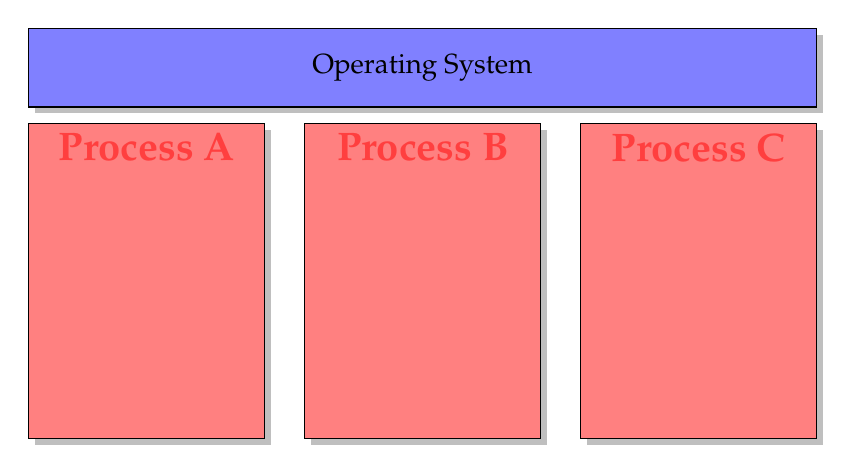
\begin{tikzpicture}[os/.style={draw,drop shadow,fill=blue!50},
                            process/.style={draw,drop shadow,fill=red!50},
                            process header/.style={font=\sc\bf\Large,red,opacity=0.5}]
            \node[os,minimum width=10cm,minimum height=1cm] (os) {Operating System};
            \coordinate (process a) at ($ (os.south west) + (0,-0.2) $);
            \coordinate (process b) at ($ (os.south west) ! 0.35 ! (os.south east) + (0,-0.2) $);
            \coordinate (process c) at ($ (os.south west) ! 0.7 ! (os.south east) + (0,-0.2) $);
            \draw[process] (process a) rectangle ++(3,-4);
            \draw[process] (process b) rectangle ++(3,-4);
            \draw[process] (process c) rectangle ++(3,-4);
            \node[anchor=north west,minimum width=3cm,process header] at (process a) {Process A};
            \node[anchor=north west,minimum width=3cm,process header] at (process b) {Process B};
            \node[anchor=north west,minimum width=3cm,process header] at (process c) {Process C};

        \end{tikzpicture}
    \end{center}
\end{frame}

\end{document}

%%% Local Variables:
%%% mode: latex
%%% TeX-master: t
%%% End:
